\documentclass[11pt,a4paper]{article}

\usepackage[margin=2.6cm]{geometry}
\usepackage{amsmath,amssymb}
\usepackage{graphicx}
\usepackage{booktabs}
\usepackage{array}
\usepackage{xcolor}
\usepackage[font=small,labelfont=bf]{caption}
\usepackage[colorlinks=true,linkcolor=blue!50!black,citecolor=blue!50!black,urlcolor=blue!50!black]{hyperref}

\newcommand{\MP}{M_{\mathrm{P}}}
\newcommand{\TJ}{T_{J}}
\newcommand{\GeV}{\,\mathrm{GeV}}
\newcommand{\code}[1]{\texttt{#1}}

\title{The kicking function in a Mathematica notebook and in the ChamPBH pipeline:\\
  an audit, and the effect of the difference on capture near $\beta = 3$}
\author{Prepared with Claude Code (Claude Opus 5.5) for D.~Seery}
\date{16 October 2026}

\begin{document}
\maketitle

\begin{abstract}
\noindent
A conformally coupled scalar field in the radiation era is pushed, or ``kicked'', whenever
the radiation is not exactly conformal, that is whenever its equation of state departs from
$w = 1/3$. Two independent codes integrate this system: a Mathematica notebook
(\code{PeakEWsurf.nb}) and a Python pipeline (ChamPBH). We compare how each one computes
the kick. The kick term is algebraically identical in the two codes. Both build the kicking
function $\Sigma(\TJ) = 1 - 3w(\TJ)$ by interpolating a table of $w$, but \emph{the tables are
not the same above $22\GeV$}. Below that temperature every shared row agrees to $10^{-12}$.
Between $22$ and $100\GeV$ the notebook's $\Sigma$ is larger by up to $10\%$. Above
$100\GeV$ the notebook keeps only four rows and forces $w = 1/3$ at $386.7\GeV$, so its
$\Sigma$ is exactly zero above that temperature; the pipeline's table continues smoothly to
$25\,\mathrm{TeV}$. The two codes also interpolate differently, but above $20\GeV$ that contributes at most
$6\times10^{-5}$ to $\Sigma$, against $4\times10^{-3}$ from the rows.

To measure the dynamical effect we re-ran the notebook's own integration with the pipeline's
$\Sigma$ substituted. This moves the coupling above which the field is captured at the
electroweak scale from $\beta = 3.00285$ to $\beta = 3.01949$. For $3.003 \lesssim \beta
\lesssim 3.019$ the histories change qualitatively. With the notebook's table they are
captured at the electroweak peak, near $\TJ \approx 52\GeV$; with the pipeline's they pass
through it and are captured at the QCD transition, near $\TJ \approx 1.64\GeV$. More than
$99\%$ of the shift comes from the table rows, and none of it comes from the interpolation.
With the pipeline's $\Sigma$ the notebook reproduces the pipeline's own capture edge,
$\beta \in (3.019, 3.020]$. Neither table records how it was made. Separately, the notebook's
closed-form matter fraction $f_m(\TJ)$ appears to have its $(1+w)$ dependence inverted.
This changes $f_m$ by up to $17\%$, but $f_m$ is at most $4\times10^{-4}$ of $\Sigma$ at the
relevant temperatures, so the error has no effect on the dynamics.
\end{abstract}

\tableofcontents

%======================================================================
\section{The system and the kick}
\label{sec:system}

\subsection{Equations of motion}

Both codes describe a scalar field $\phi$ in the Einstein frame, coupled to matter and
radiation through the Jordan-frame metric $\tilde g_{\mu\nu} = A^2(\phi)\, g_{\mu\nu}$, with
\begin{equation}
  A(\phi) = \exp(\beta\phi/\MP),
\end{equation}
where $\MP = 2.43\times10^{18}\GeV$ is the reduced Planck mass. Below we set $\MP = 1$. The
potential is $V(\phi) = v_0^4 \exp(M/\phi)$. Matter and radiation are minimally coupled to
$\tilde g$, so their Jordan-frame temperature $\TJ$ obeys the usual thermodynamics. The radiation
density is $\tilde\rho_r = (\pi^2/30)\, g_\rho(\TJ)\, \TJ^4$, its Einstein-frame density is
$\rho_r = A^4 \tilde\rho_r$, and $w(\TJ) = \tilde p_r/\tilde\rho_r$ is its equation of state.
Let $f_m = \rho_m/\rho_r$ be the matter fraction and $y = \mathrm{d}\phi/\mathrm{d}N$, where
$N$ counts Einstein-frame e-folds. The Friedmann equation is
\begin{equation}
  3H^2 = \frac{\rho_r(1+f_m) + V}{1 - y^2/6}.
  \label{eq:friedmann}
\end{equation}
The field is sourced by the trace of the matter stress tensor:
\begin{equation}
  \ddot\phi + 3H\dot\phi + V'(\phi) = -\frac{\mathrm{d}\ln A}{\mathrm{d}\phi}\, T^{\mu}{}_{\mu}
  = -\beta\left(\rho_r - 3p_r + \rho_m\right)
  = -\beta\rho_r\left(\Sigma + f_m\right),
\end{equation}
where
\begin{equation}
  \boxed{\;\Sigma(\TJ) \equiv 1 - 3w(\TJ)\;}
\end{equation}
is the \emph{kicking function}. It vanishes for conformal radiation and becomes positive
whenever a species becomes non-relativistic or the plasma passes through a transition. In the
Standard Model it has three peaks, at $e^\pm$ annihilation ($\TJ \approx 0.16\,\mathrm{MeV}$),
at the QCD crossover ($\approx 0.18\GeV$) and at the electroweak scale ($\approx 53\GeV$)
(Fig.~\ref{fig:sigma}a). Written in e-folds, the kick is the term
\begin{equation}
  \left.\frac{\mathrm{d}y}{\mathrm{d}N}\right|_{\text{kick}}
  = -\frac{\beta\rho_r(\Sigma + f_m)}{H^2}
  = -3\left(1 - \frac{y^2}{6}\right)\frac{\beta\rho_r\,(\Sigma + f_m)}{\rho_r(1+f_m) + V}.
  \label{eq:kick}
\end{equation}
The Jordan-frame temperature follows from entropy conservation in the Jordan frame,
\begin{equation}
  \frac{\mathrm{d}\ln\TJ}{\mathrm{d}N} = -\frac{1 + \beta y}{1 + \tfrac13\,\mathrm{d}\ln g_s/\mathrm{d}\ln\TJ}.
  \label{eq:TJ}
\end{equation}
So $\TJ$ \emph{stops falling and turns round} wherever $1 + \beta y = 0$. If the kick drives
$y$ below $-1/\beta$ near a peak of $\Sigma$, then $\TJ$ reaches a minimum and stays near
that peak. In this report a history is \emph{captured} at a peak if $\TJ$ has a minimum
there. In particular, a history is captured at the electroweak scale if its first $\TJ$
minimum lies above $20\GeV$. This is an operational criterion, chosen for this comparison;
it is not the pipeline's own classification. For $\beta$ close to $3$ the outcome is
delicate, because $y$ then hovers near $-1/\beta$ for many e-folds.

\subsection{How the two codes write the kick}

\paragraph{Notebook.}
The notebook integrates $(\phi, y, \ln\TJ)$ with Mathematica's \code{NDSolve}. The right-hand
side for $y$ contains the term
\begin{verbatim}
  -3 (1 - y^2/6) (Vp + beta rho (Sigma[T] + fmTinterp[T]))
                    / (rho (1 + fmTinterp[T]) + V)
\end{verbatim}
which is Eq.~\eqref{eq:kick} together with the potential gradient. Here \code{rho} is computed
from $\TJ$ at each step as $A^4(\pi^2/30)g_\rho\TJ^4$. The notebook defines
\code{Sigma[T] = 1 - 3 w[T]}, with $w$ taken from a table (\S\ref{sec:tables}), and $f_m$
from a closed-form expression (\S\ref{sec:fm}).

\paragraph{Pipeline.}
The pipeline integrates $(\phi, y, \ln\rho_r, \ln f_m, \ln\TJ)$. Its kick term is
\begin{equation}
  \left.\frac{\mathrm{d}y}{\mathrm{d}N}\right|_{\text{kick}}
  = -3E\,\beta\,\frac{\Sigma + f_m}{1 + f_m},
  \qquad
  E = 1 - \frac{y^2}{6} - \frac{V}{3H^2},
\end{equation}
with $\Sigma = 1 - 3w(\TJ)$ evaluated from its own table. By Eq.~\eqref{eq:friedmann},
$E = \rho_r(1+f_m)/3H^2$. Mathematica's \code{Simplify} reduces the difference between this
and Eq.~\eqref{eq:kick} to exactly zero.

\medskip\noindent
\textbf{Conclusion 1.} \emph{The kick has the same functional form in both codes.} Any
difference must come from the inputs: $\Sigma(\TJ)$ and $f_m(\TJ)$.

%======================================================================
\section{The tables behind \texorpdfstring{$\Sigma(\TJ)$}{Sigma(T\_J)}}
\label{sec:tables}

\subsection{What each code tabulates}

\begin{table}[ht]
\centering\footnotesize
\begin{tabular}{@{}>{\raggedright\arraybackslash}p{2.3cm}>{\raggedright\arraybackslash}p{6.0cm}>{\raggedright\arraybackslash}p{5.6cm}@{}}
\toprule
 & Notebook & Pipeline \\
\midrule
Rows & 132 & 189 \\
Range of rows & $3.65\times10^{-5}$ -- $386.7\GeV$ & $10^{-5}$ -- $2.51\times10^{4}\GeV$ \\
Spacing & $0.05$ dex to $100\GeV$, then rows at $158$, $251$, $316$ and $386.7\GeV$ & $0.05$ dex throughout \\
End rows & $w = 1/3$ exactly at both ends, off the $0.05$-dex grid & on the grid \\
Outside the rows & $w = 1/3$ & $w = 1/3$ \\
Interpolation & Mathematica \code{Interpolation} (order 3) of $\ln w$ against $\ln T$:
  piecewise local cubics, continuous &
  cubic B-spline of $w$ against $\ln T$ (\code{scipy} \code{make\_interp\_spline}), $C^2$ \\
\bottomrule
\end{tabular}
\caption{The two tabulations of $w(\TJ)$.}
\label{tab:tables}
\end{table}

Table~\ref{tab:tables} summarises the two tables. Of the notebook's 132 rows, 130 lie on the
pipeline's $0.05$-dex grid. The other two are its end points, where $w = 1/3$ appears to have
been imposed by hand. Of the 130 shared rows, \textbf{113 agree to $10^{-12}$}: every shared row
below $22\GeV$. The 17 that differ are listed in Table~\ref{tab:rows}. From $25$ to $100\GeV$
the notebook's $\Sigma$ is larger than the pipeline's by $1$--$10\%$, the gap growing with
temperature. Above $100\GeV$ the notebook has only three interior rows, which disagree with the
pipeline's in both directions. Its final row then forces $w$ back to $1/3$ at $386.7\GeV$.
The pipeline's $\Sigma$ instead decays smoothly, from $3.4\times10^{-3}$ at $398\GeV$ to
$6\times10^{-4}$ at $1\,\mathrm{TeV}$ and $10^{-6}$ at $25\,\mathrm{TeV}$.

\begin{table}[ht]
\centering\small
\begin{tabular}{@{}rrrr@{\hspace{2.5em}}rrrr@{}}
\toprule
$T$ [GeV] & $\Sigma_{\rm nb}$ & $\Sigma_{\rm pipe}$ & $\Delta\Sigma$ &
$T$ [GeV] & $\Sigma_{\rm nb}$ & $\Sigma_{\rm pipe}$ & $\Delta\Sigma$ \\
\midrule
 22.39 & 0.01888 & 0.01885 & $+0.00004$ &  63.10 & 0.03717 & 0.03638 & $+0.00079$ \\
 25.12 & 0.02253 & 0.02225 & $+0.00028$ &  70.79 & 0.03603 & 0.03477 & $+0.00127$ \\
 28.18 & 0.02620 & 0.02567 & $+0.00053$ &  79.43 & 0.03438 & 0.03251 & $+0.00187$ \\
 31.62 & 0.02968 & 0.02917 & $+0.00051$ &  89.13 & 0.03227 & 0.02987 & $+0.00240$ \\
 35.48 & 0.03274 & 0.03220 & $+0.00054$ & 100.00 & 0.02978 & 0.02697 & $+0.00281$ \\
 39.81 & 0.03517 & 0.03472 & $+0.00044$ & 158.49 & 0.01721 & 0.01559 & $+0.00161$ \\
 44.67 & 0.03678 & 0.03649 & $+0.00030$ & 251.19 & 0.00506 & 0.00768 & $-0.00263$ \\
 50.12 & 0.03761 & 0.03732 & $+0.00029$ & 316.23 & 0.00121 & 0.00519 & $-0.00398$ \\
 56.23 & 0.03772 & 0.03733 & $+0.00039$ & 386.7 & 0 (imposed) & 0.00363$^\ast$ & \\
\bottomrule
\end{tabular}
\caption{The shared table rows that differ, with $\Delta\Sigma = \Sigma_{\rm nb} -
\Sigma_{\rm pipe}$. The notebook's $386.7\GeV$ row is not on the pipeline's grid. The value
marked $^\ast$ is the pipeline's interpolant there.}
\label{tab:rows}
\end{table}

\begin{figure}[p]
\centering
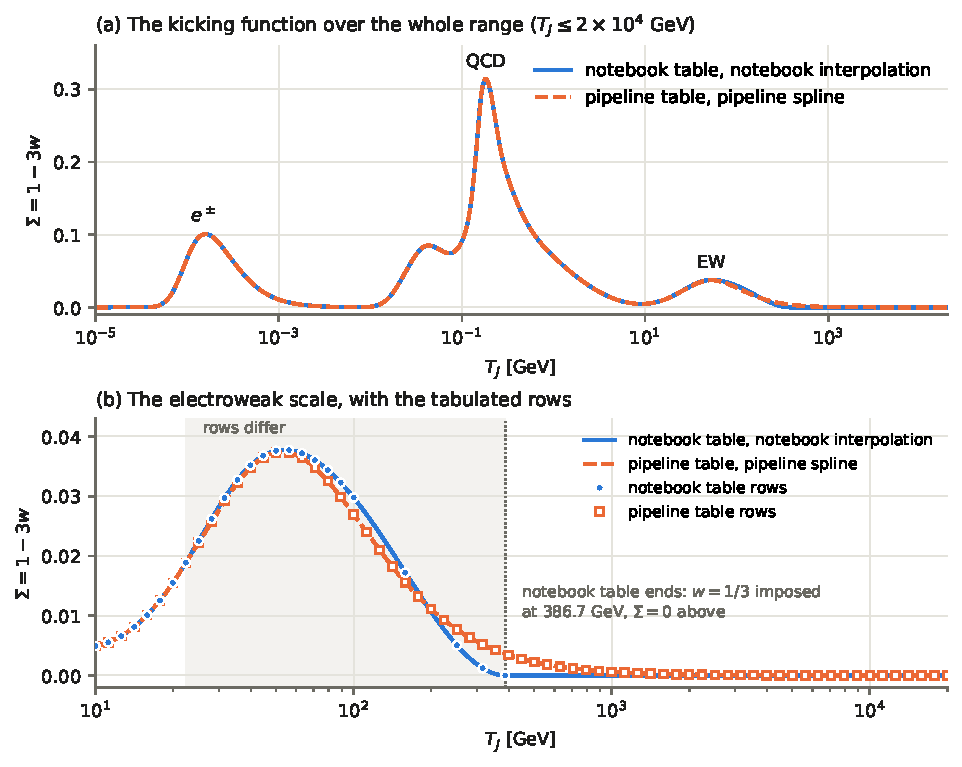
\includegraphics[width=\textwidth]{figures/sigma_overview.pdf}
\caption{The kicking function $\Sigma = 1 - 3w$ in the two codes. (a)~Over the whole range the
two curves are indistinguishable at this scale. (b)~At the electroweak scale they are not. The
markers are the rows each code tabulates. The shaded band marks where shared rows differ, and
the dotted line marks the notebook's last row, where $w = 1/3$ is imposed.}
\label{fig:sigma}
\end{figure}

\subsection{Peaks and integrated kick}

Table~\ref{tab:peaks} compares the three peaks and the integral $\int\Sigma\,\mathrm{d}\ln\TJ$
over each. The integral is a rough measure of the total kick a peak delivers. At $e^\pm$
annihilation and the QCD crossover the two codes agree to $0.1\%$ or better. At the
electroweak scale the notebook's peak is $0.9\%$ higher and $1.6\%$ hotter. Between $20$ and
$386.7\GeV$ its integral is $1.0\%$ larger. Above $386.7\GeV$ the notebook delivers no kick,
where the pipeline delivers $0.0019$. Over $20\GeV$--$20\,\mathrm{TeV}$ as a whole, the
notebook's integral is therefore $1.8\%$ \emph{smaller} (0.0673 against 0.0685).

\begin{table}[ht]
\centering\footnotesize
\begin{tabular}{@{}lcccc@{}}
\toprule
Peak & \multicolumn{2}{c}{$\Sigma_{\max}$ (at $\TJ$)} & \multicolumn{2}{c}{$\int\Sigma\,\mathrm{d}\ln\TJ$} \\
 & Notebook & Pipeline & Notebook & Pipeline \\
\midrule
$e^\pm$ ($10^{-5}$--$2\times10^{-3}\GeV$) & 0.10074 ($0.1607\,\mathrm{MeV}$) & 0.10073 ($0.1603\,\mathrm{MeV}$) & 0.16087 & 0.16099 \\
QCD ($2\times10^{-3}$--$1\GeV$) & 0.31448 ($0.1820\GeV$) & 0.31453 ($0.1820\GeV$) & 0.50823 & 0.50821 \\
EW ($10$--$386.7\GeV$) & 0.03776 ($54.08\GeV$) & 0.03744 ($53.21\GeV$) & 0.07346 & 0.07277 \\
Above $386.7\GeV$ (to $2\times10^4\GeV$) & 0 & 0.00362 ($387\GeV$) & 0 & 0.00192 \\
\bottomrule
\end{tabular}
\caption{Peaks of $\Sigma$ and its integral over $\ln\TJ$, evaluated on a grid of 1000 points
per decade.}
\label{tab:peaks}
\end{table}

\subsection{Is it the data or the interpolation?}
\label{sec:data-vs-scheme}

The two codes differ in both their rows and their interpolation scheme. We separated the two
effects by interpolating each table with the \emph{other} code's scheme. This gives four
versions of $\Sigma$: two sets of rows, each with two schemes. Figure~\ref{fig:dvs} shows the
largest $|\Delta\Sigma|$ in each $0.05$-dex interval when one ingredient is changed and the
other is held fixed:
\begin{itemize}
\item \textbf{Changing the rows} (black) moves $\Sigma$ by up to $4.1\times10^{-3}$
  (at $337\GeV$) between $20$ and $386.7\GeV$, and by up to $3.6\times10^{-3}$ above
  $386.7\GeV$. The result is the same whichever scheme is held fixed. Below $10\GeV$ the
  only change is near $40\,\mathrm{keV}$, where the notebook's imposed lower end point
  replaces the pipeline's rows (up to $5\times10^{-4}$, well below the $e^\pm$ peak).
\item \textbf{Changing the interpolation} moves $\Sigma$ by at most $1.1\times10^{-5}$ on the
  pipeline's rows and $5.5\times10^{-5}$ on the notebook's sparser rows, anywhere above
  $20\GeV$. The interpolants agree at every row and differ only between rows. The largest
  scheme difference anywhere is $1.3\times10^{-3}$, at $0.167\GeV$ on the steep side of the
  QCD peak. The QCD integral is unchanged to $2\times10^{-5}$, and \S\ref{sec:attribution} shows that
  this difference has no dynamical effect.
\end{itemize}
Over $20\GeV$--$20\,\mathrm{TeV}$ the integral $\int\Sigma\,\mathrm{d}\ln\TJ$ is
$0.06731 / 0.06729$ for the notebook's rows (notebook / pipeline scheme) and $0.06854 / 0.06854$
for the pipeline's.

\begin{figure}[ht]
\centering
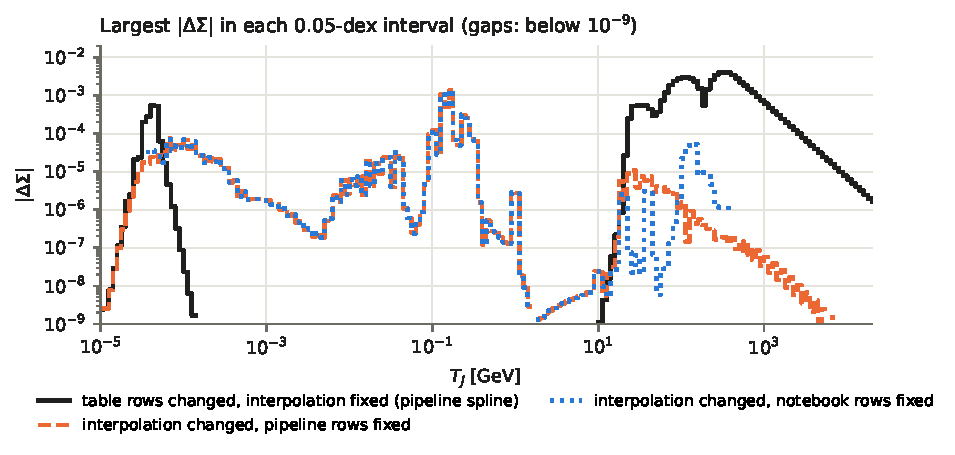
\includegraphics[width=\textwidth]{figures/sigma_data_vs_scheme.pdf}
\caption{Each curve changes one ingredient of $\Sigma$ and holds the other fixed. The changed
ingredient is either the table rows (black) or the interpolation scheme (dashed and dotted).
Above $20\GeV$ the rows matter 75 to 400 times more than the scheme.}
\label{fig:dvs}
\end{figure}

\medskip\noindent
\textbf{Conclusion 2.} \emph{The two codes' $\Sigma(\TJ)$ differ at the electroweak scale
because their tables differ, not because they interpolate differently.}

%======================================================================
\section{The matter fraction}
\label{sec:fm}

The kick is sourced by $\Sigma + f_m$, so we also compared $f_m$. The notebook uses the closed
form
\begin{equation}
  f_m^{\rm nb}(\TJ) = \frac{2.78\times10^{-9}\GeV}{3\,\TJ\,\bigl(1 + w(\TJ)\bigr)},
  \label{eq:fm-nb}
\end{equation}
tabulated with linear interpolation on a $10^{-4}$-dex grid. The pipeline instead evolves
$\ln f_m$, with $\mathrm{d}\ln f_m/\mathrm{d}N = (1-\Sigma)(1+\beta y)$. Its starting value is
$f_m = \rho_{m0}(1+z)^3/\tilde\rho_r(\TJ)$, where $1+z$ follows from conservation of
$\TJ\,g_s^{1/3}$. For the comparison we evaluate the pipeline's $f_m$ from that starting
formula at each $\TJ$, i.e.\ at fixed field.

For a single-temperature plasma, $\tilde\rho_r + \tilde p_r = \TJ s$, which gives
\begin{equation}
  f_m = \frac{\rho_m}{s}\,\frac{1 + w}{\TJ},
  \qquad \frac{\rho_m}{s} \simeq 5.2\times10^{-10}\GeV \text{ (Planck 2018)}.
\end{equation}
Equation~\eqref{eq:fm-nb} agrees with this at $w = 1/3$, since
$2.78\times10^{-9}/4 = 6.95\times10^{-10} = \tfrac43 \times 5.2\times10^{-10}$. Its
$w$-dependence, however, is \emph{the inverse} of the one expected: it divides by $(1+w)$ where
the thermodynamic result multiplies by it. Relative to the expected form, the notebook's $f_m$
is too large by $(16/9)/(1+w)^2$, about $1.18$ at the QCD peak. Figure~\ref{fig:fm}a shows the
ratio of the two codes' $f_m$. It ranges from $0.87$ (at $10\,\mathrm{keV}$, where the notebook
also omits $g_s \ne g_\rho$ after neutrino decoupling) to $1.17$ (at $0.19\GeV$).

The error does not matter here. Figure~\ref{fig:fm}b shows that $f_m/\Sigma$ is at most
$3.6\times10^{-4}$ between $0.1\,\mathrm{MeV}$ and $386\GeV$, at the trough near
$7\,\mathrm{MeV}$, and is $10^{-8}$--$10^{-10}$ at the QCD and electroweak peaks. Above
$386.7\GeV$, $f_m$ is the notebook's \emph{only} source of kick, but it is
between $2\times10^{-12}$ and $3\times10^{-14}$ there. The pipeline's $\Sigma$ is
$3.6\times10^{-3}$ at $387\GeV$ and still $1.6\times10^{-6}$ at $20\,\mathrm{TeV}$. All the runs in
\S\ref{sec:dynamics} keep the notebook's own $f_m$.

\begin{figure}[ht]
\centering
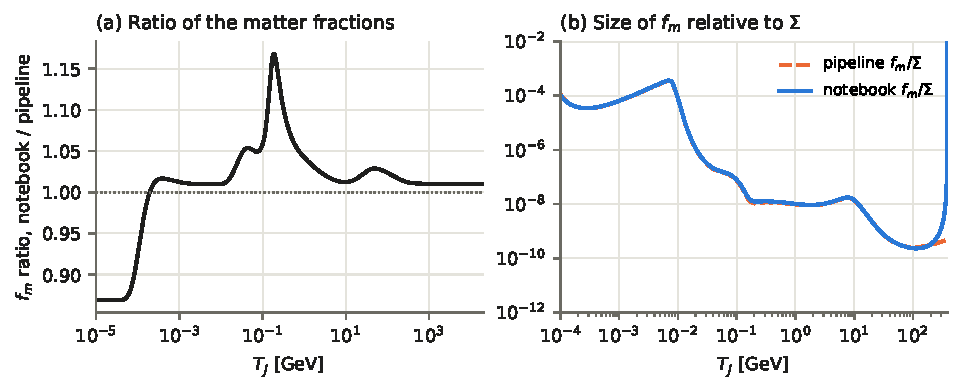
\includegraphics[width=\textwidth]{figures/fm.pdf}
\caption{(a)~The notebook's matter fraction relative to the pipeline's. (b)~The matter fraction
as a fraction of $\Sigma$. Above $300\GeV$ the notebook's curve rises because its $\Sigma$
falls to zero.}
\label{fig:fm}
\end{figure}

%======================================================================
\section{Dynamical effect near \texorpdfstring{$\beta = 3$}{beta = 3}}
\label{sec:dynamics}

\subsection{Method}

We re-ran the notebook's own integration, changing nothing but $\Sigma$. All other definitions
were evaluated directly from the notebook's input cells by a Mathematica 15.0.1 kernel, without
transcription. These include the effective degrees of freedom $g_\rho$ and $g_s$, $f_m$,
$V$ and $\rho_r(\TJ)$. The integrator settings are also the notebook's: \code{NDSolve} with
\code{StiffnessSwitching}, accuracy and precision goals of 10, and \code{MaxStepSize}
$10^{-3}$. Every run starts at $\TJ = 2\times10^4\GeV$ with $y = 0$, and stops when $\phi$
falls to $0.1\,\MP$ or at $N = 150$. The parameters are those of the notebook: $\phi_i =
10\,\MP$ (and $100\,\MP$ for one run), $M = 10^{-2}\,\MP$ and $v_0 = 2.16\times10^{-12}\GeV$.

Four versions of $\Sigma$ were used:
\begin{center}\small
\begin{tabular}{@{}ll@{}}
\toprule
\code{nb} & the notebook's $\Sigma$, unchanged \\
\code{pipe} & the pipeline's $\Sigma$ everywhere \\
\code{ew} & the notebook's $\Sigma$ below $20\GeV$, the pipeline's above (the two agree to $3\times10^{-6}$ at $20\GeV$) \\
\code{csvnb} & the pipeline's rows, interpolated the notebook's way \\
\bottomrule
\end{tabular}
\end{center}
The pipeline's $\Sigma$ was evaluated by its own code, sampled at 1000 points per decade, and
passed to Mathematica as a cubic interpolant in $\ln\TJ$. That interpolant differs from the
pipeline's own values by at most $9.4\times10^{-9}$, measured at the midpoints between samples.
Turning points of $\TJ$ are the zeros of $1+\beta y$, located with \code{FindRoot}.

\subsection{Results}

Table~\ref{tab:scan} and Figs.~\ref{fig:hist}--\ref{fig:threshold} give the results. In the
window $3.003 \lesssim \beta \lesssim 3.019$ the outcome changes qualitatively. With the
notebook's $\Sigma$ the field is captured at the electroweak peak: $\TJ$ reaches a minimum
of $51$--$53\GeV$ within $9$--$12$ e-folds and then stays at that scale. With the pipeline's
$\Sigma$ the history passes through the electroweak scale and is captured at the QCD
transition, reaching a minimum of $1.64$--$1.65\GeV$ $15$ to $24$ e-folds later. The integration
also runs about $3.5$ e-folds longer before $\phi$ reaches $0.1\,\MP$.

Outside the window the type of capture is the same, but the details move. Above it, the
pipeline's $\Sigma$ gives a minimum $3.5$--$4\GeV$ colder ($49$--$51\GeV$ against
$53$--$54\GeV$), $0.8$--$2.8$ e-folds later. Below it, both are captured at QCD at the same
temperature, $1.626$--$1.631\GeV$, but the notebook's history arrives $6$--$9$ e-folds later.
At $\beta = 3.000$ the notebook's history has no minimum at all before $\phi$ reaches
$0.1\,\MP$; it ends at $\TJ = 22.8\GeV$, still falling slowly.

\begin{table}[ht]
\centering\small
\begin{tabular}{@{}c@{\hspace{1.2em}}lrr@{\hspace{1.5em}}lrr@{}}
\toprule
 & \multicolumn{3}{c}{Notebook $\Sigma$} & \multicolumn{3}{c}{Pipeline $\Sigma$} \\
\cmidrule(lr){2-4}\cmidrule(l){5-7}
$\beta$ & first minimum & $N$ & $N_{\rm end}$ & first minimum & $N$ & $N_{\rm end}$ \\
\midrule
2.990 & QCD, $1.626\GeV$ & 29.16 & 38.93 & QCD, $1.626\GeV$ & 22.91 & 38.93 \\
2.995 & QCD, $1.631\GeV$ & 32.87 & 38.98 & QCD, $1.631\GeV$ & 23.81 & 38.98 \\
3.000 & none (ends at $22.8\GeV$) & -- & 36.56 & QCD, $1.636\GeV$ & 24.97 & 39.03 \\
3.005 & \textbf{EW}, $51.31\GeV$ & 11.30 & 35.68 & \textbf{QCD}, $1.641\GeV$ & 26.59 & 39.07 \\
3.010 & \textbf{EW}, $52.06\GeV$ & 10.28 & 35.65 & \textbf{QCD}, $1.646\GeV$ & 29.09 & 39.12 \\
3.015 & \textbf{EW}, $52.68\GeV$ & 9.84 & 35.67 & \textbf{QCD}, $1.651\GeV$ & 34.08 & 39.15 \\
3.020 & EW, $53.24\GeV$ & 9.55 & 35.70 & EW, $49.36\GeV$ & 12.37 & 35.90 \\
3.025 & EW, $53.77\GeV$ & 9.34 & 35.73 & EW, $50.15\GeV$ & 10.48 & 35.82 \\
3.030 & EW, $54.26\GeV$ & 9.17 & 35.76 & EW, $50.77\GeV$ & 9.97 & 35.85 \\
\bottomrule
\end{tabular}
\caption{The first $\TJ$ minimum and the e-fold at which it occurs, for $\phi_i = 10\,\MP$.
$N_{\rm end}$ is where $\phi$ reaches $0.1\,\MP$. The bold rows change their type of capture.}
\label{tab:scan}
\end{table}

\begin{figure}[ht]
\centering
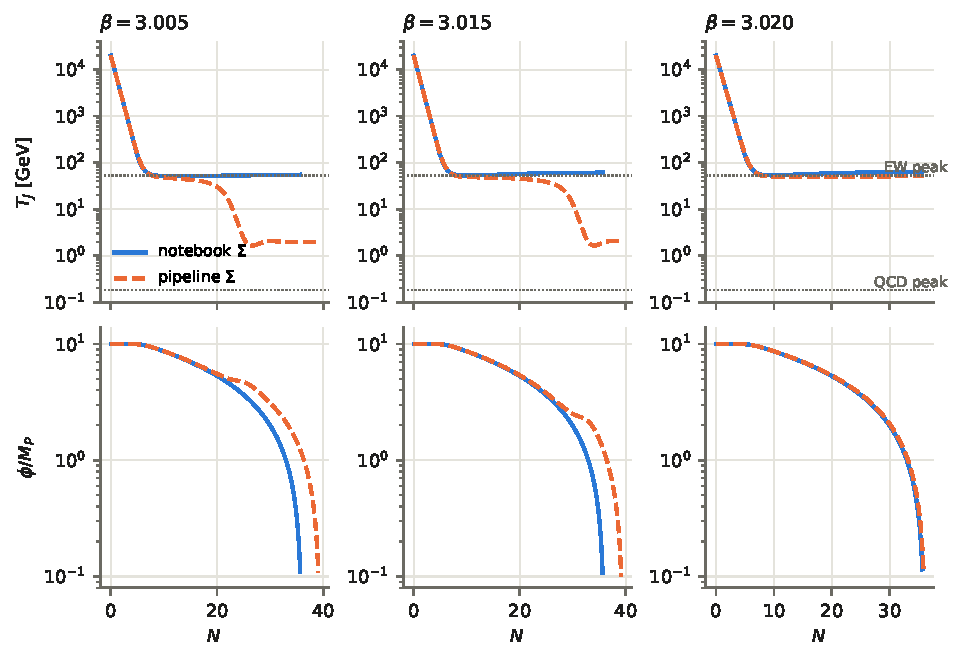
\includegraphics[width=\textwidth]{figures/histories.pdf}
\caption{$\TJ(N)$ (top) and $\phi(N)$ (bottom) for three couplings, from the notebook's
integration with its own $\Sigma$ (solid) and with the pipeline's (dashed). At
$\beta = 3.005$ and $3.015$ the notebook's history is captured at the electroweak scale and the
pipeline-$\Sigma$ history at QCD. At $\beta = 3.020$ both are captured at the electroweak scale.}
\label{fig:hist}
\end{figure}

\paragraph{The threshold.}
We bisected in $\beta$, to a tolerance of $10^{-4}$, for the smallest coupling captured at the
electroweak scale:
\begin{center}\small
\begin{tabular}{@{}lll@{}}
\toprule
Rows & Interpolation & Electroweak-capture threshold \\
\midrule
notebook & notebook & $\beta_c \in (3.002813,\ 3.002891)$ \\
pipeline & notebook & $\beta_c \in (3.019375,\ 3.019453)$ \\
pipeline & pipeline & $\beta_c \in (3.019453,\ 3.019531)$ \\
\bottomrule
\end{tabular}
\end{center}
Substituting the pipeline's $\Sigma$ raises the threshold by $\Delta\beta_c = +0.0167$. Changing
the interpolation with the rows held fixed moves it by less than $1.6\times10^{-4}$, under
$1\%$ of the total. Just below each threshold there is a band of $\beta$ in which no
$\TJ$ minimum occurs before the integration stops (the open markers in
Fig.~\ref{fig:threshold}). With the notebook's $\Sigma$ the band includes
$\beta = 3.000$--$3.0028$; with the pipeline's it includes $\beta = 3.0175$--$3.0194$. We did
not map its lower edge.

The pipeline's own fine scan of capture near $\beta = 3$ places its electroweak-capture edge
in $(3.019, 3.020]$. That scan used a different potential ($\phi_i = 5\,\MP$,
$M = 10^{-3}\,\MP$, $\Lambda = 1\,\mathrm{meV}$) and the pipeline's own integrator. The
notebook run with the pipeline's $\Sigma$ falls inside that bracket. This suggests that the
threshold is fixed mainly by $\Sigma$, and that the two integrators otherwise agree here.

\begin{figure}[ht]
\centering
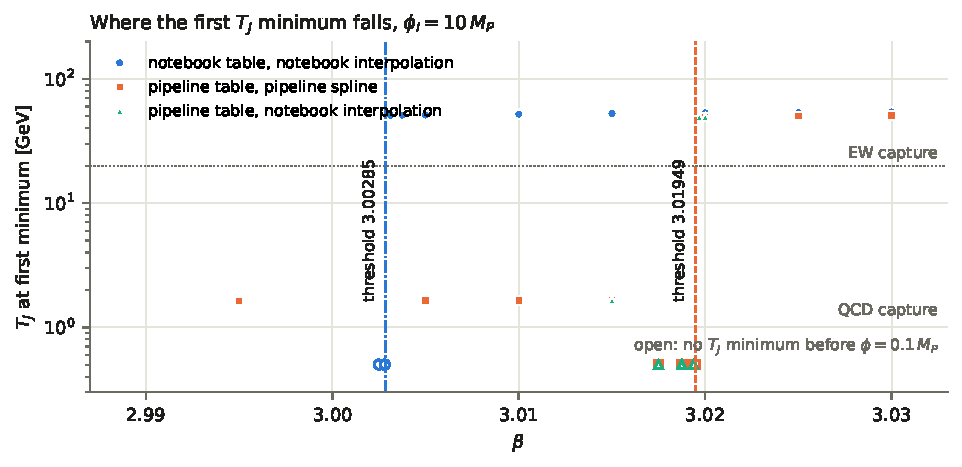
\includegraphics[width=\textwidth]{figures/threshold.pdf}
\caption{The temperature of the first $\TJ$ minimum against $\beta$, from the scan and the
bisection runs. Filled markers above $20\GeV$ are electroweak captures and those near
$1.6\GeV$ are QCD captures. Open markers are histories with no minimum before $\phi$ reaches
$0.1\,\MP$. The vertical lines are the two thresholds.}
\label{fig:threshold}
\end{figure}

\paragraph{A longer history.}
The notebook also integrates $\phi_i = 100\,\MP$ at $\beta = 3.005$ out to $N = 150$
(Fig.~\ref{fig:phi100}). With either $\Sigma$, $\TJ$ first turns at the electroweak scale,
with a minimum at $N \approx 9$--$10$, and reaches a maximum at $N \approx 83$. With the
notebook's $\Sigma$ the history then stays near the electroweak scale, ending at $58\GeV$.
With the pipeline's $\Sigma$, $\TJ$ falls away after the maximum, and the history is
captured at QCD ($1.64\GeV$ at $N = 134$).

\begin{figure}[ht]
\centering
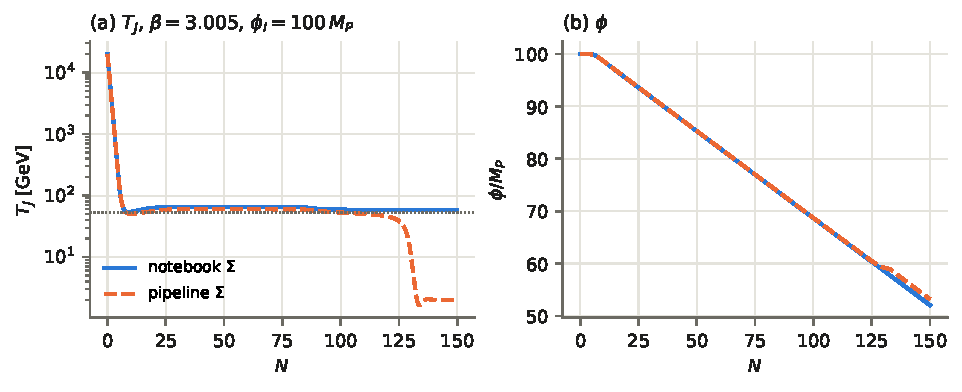
\includegraphics[width=\textwidth]{figures/phi100.pdf}
\caption{The notebook's $\phi_i = 100\,\MP$, $\beta = 3.005$ history with each $\Sigma$.}
\label{fig:phi100}
\end{figure}

\subsection{Attribution, controls and convergence}
\label{sec:attribution}

\begin{itemize}
\item \textbf{The electroweak table is responsible.} The \code{ew} variant uses the notebook's
  $\Sigma$ below $20\GeV$, including its interpolation at the QCD and $e^\pm$ peaks. Over all
  nine couplings of the scan it reproduces the \code{pipe} histories to
  $|\Delta\ln\TJ| \le 1.5\times10^{-5}$ and $|\Delta\phi| \le 5\times10^{-6}\,\MP$. So the
  $1.3\times10^{-3}$ scheme difference on the side of the QCD peak has no effect.
\item \textbf{The rows are responsible, not the scheme.} The \code{csvnb} threshold lies within
  $1.6\times10^{-4}$ of the \code{pipe} threshold, against a total shift of $0.0167$.
\item \textbf{The substitution is faithful.} Replacing the notebook's definition of
  $\Sigma$ with the substituted copy (variant \code{nb}) changes the unmodified notebook's
  histories by $|\Delta\ln\TJ| \le 6\times10^{-6}$ at $\beta = 3.000$ and $6\times10^{-8}$ at
  $\beta = 3.015$.
\item \textbf{The integrations are converged.} Reducing \code{MaxStepSize} from $10^{-3}$ to
  $10^{-4}$ at $\beta = 3.015$ changes $\ln\TJ$ by at most $9\times10^{-8}$ (\code{nb}) and
  $7\times10^{-6}$ (\code{ew}). It changes no turning point and no end point.
\end{itemize}

\medskip\noindent
\textbf{Conclusion 3.} \emph{The table difference above $22\GeV$ moves the
electroweak-capture threshold by $+0.0167$ in $\beta$, and changes the type of capture for
$3.003 \lesssim \beta \lesssim 3.019$. With the pipeline's table, the notebook reproduces the
pipeline's own capture edge.}

%======================================================================
\section{Provenance, and which table to trust}
\label{sec:provenance}

Neither code records how its table was made. The pipeline's table was added without the
script or method that produced it. It is described as the Saikawa--Shirai equation of state
(arXiv:1803.01038) ``with adjustments''. Its lack of provenance is already an open issue in
the pipeline's records. The notebook's table matches it row for row up to $22\GeV$, so the
two evidently share a source. Above $22\GeV$ they diverge, and the notebook's rows also
disagree with the unadjusted Saikawa--Shirai $w$. The pipeline keeps that $w$ in a
code-comparison table, where it agrees with the pipeline's Saikawa--Shirai implementation to
$8\times10^{-8}$ above $10\,\mathrm{MeV}$. Its $\Sigma$ is $0.0052$ at $398\GeV$.

Two judgements follow. Neither has been tested beyond what is stated.
\begin{enumerate}
\item \emph{The notebook's tail is unlikely to be physical.} At $T \approx 400\GeV$ the top
  quark, Higgs, $W$ and $Z$ are still massive enough to make $\Sigma \sim 10^{-3}$. The
  running couplings add a trace anomaly that continues above that temperature. A $w$ that
  reaches $1/3$ exactly at $386.7\GeV$ and stays there looks like a truncation, not a physical
  feature. Both the pipeline's adjusted table and the unadjusted Saikawa--Shirai $w$ have a
  smooth tail there.
\item \emph{We cannot tell which version of the $25$--$100\GeV$ rows is intended.} The
  notebook's rows are $1$--$10\%$ higher there. They may be a different revision of the same
  adjusted table.
\end{enumerate}
We have not separated how much of the threshold shift comes from the $25$--$386.7\GeV$ rows
and how much from the missing tail above $386.7\GeV$. The two pull in opposite directions in
$\int\Sigma\,\mathrm{d}\ln\TJ$ (Table~\ref{tab:peaks}), and capture is not decided by the
integral alone, so the split needs a separate run.

%======================================================================
\section{Summary and recommendations}

\begin{enumerate}
\item The kick term is the same in both codes (\S\ref{sec:system}).
\item The kicking function differs above $22\GeV$, because the tables differ (\S\ref{sec:tables}).
  The interpolation schemes contribute at most $6\times10^{-5}$ there.
\item This moves the electroweak-capture threshold from $\beta = 3.00285$ (notebook) to
  $3.01949$ (pipeline). In between, histories that the notebook captures at the electroweak
  scale are captured at QCD (\S\ref{sec:dynamics}).
\item The notebook's closed-form $f_m$ appears to have its $(1+w)$ factor inverted
  (\S\ref{sec:fm}). The error is dynamically irrelevant here, but should be fixed before the
  form is reused.
\end{enumerate}

\noindent We recommend:
\begin{itemize}
\item Use one $w(\TJ)$ table in both codes, with a recorded origin. Until then, results near
  the electroweak-capture edge should be quoted together with the table that produced them.
\item Find out where the notebook's electroweak rows and its $386.7\GeV$ end point came from.
  If the truncation was deliberate, record why.
\item Run the split described in \S\ref{sec:provenance}, which needs about three bisections.
\item Correct Eq.~\eqref{eq:fm-nb} to $f_m = (\rho_m/s)(1+w)/\TJ$, or replace it with the
  pipeline's treatment, which also includes $g_s \neq g_\rho$.
\end{itemize}

\paragraph{Not covered.}
This report compares only $\Sigma$, $f_m$ and the form of the kick. It does not compare the two
codes' $g_\rho$ and $g_s$, the $\TJ$ equation~\eqref{eq:TJ}, the friction term, or the
treatment of $\rho_r$ (algebraic in $\TJ$ in the notebook, integrated in the pipeline). All
the runs use the notebook's integrator and parameters; the pipeline's integrator was not run.

%======================================================================
\appendix
\section{Reproducing these results}

\paragraph{Versions.}
\begin{itemize}
\item Notebook \code{PeakEWsurf.nb}, not under version control. Its SHA-256 is\\
  {\small\code{5bd78e6f43b6b7fc4a2eaff746263b63a66c27786eef76cea90edbdd070e92e4}}.
\item ChamPBH at commit \code{c21cdfb}.
\item Mathematica 15.0.1 (macOS, ARM); Python 3.13.16 with NumPy 2.3.5, SciPy 1.17.0,
  pandas 3.0.0 and Matplotlib 3.10.8.
\end{itemize}

\paragraph{Files.}
Everything is in \code{.documents/peakewsurf-kicking-function/}:
\begin{itemize}
\item \code{scripts/nb\_kick.wls}: evaluates the notebook's definitions and exports its $w$
  table, $\Sigma$ and $f_m$ on a grid, together with the symbolic check of \S\ref{sec:system}.
\item \code{scripts/compare\_kick.py}: evaluates the pipeline's $\Sigma$ and $f_m$ on the same
  grid. It replaces \code{datastorekit} with a stub because only the EOS is needed.
\item \code{scripts/sigma\_cross.wls}: interpolates the pipeline's rows with the notebook's scheme.
\item \code{scripts/swap\_defs.wl}, \code{swap\_runs.wls}, \code{bisect.wls}: the integrations
  and the bisection.
\item \code{scripts/compare\_runs.py}, \code{build\_data.py}, \code{make\_figures.py}: the
  analysis, the data products and the figures.
\item \code{data/}: the notebook's table, the $\Sigma$/$f_m$ grid at 200 points per decade,
  the row-by-row comparison, the downsampled histories, \code{runs\_summary.json} (every run's
  turning points) and \code{stats.json} (every number quoted here, at full resolution).
\end{itemize}

\paragraph{Commands.}
Run from the repository root. \code{WORK} is a scratch directory, and \code{NB} is the
notebook's absolute path. \code{wolframscript} must be told where the kernel is.
{\small
\begin{verbatim}
APP="/Applications/Mathematica 15/Wolfram.app"
export WolframKernel="$APP/Contents/MacOS/WolframKernel"
D=.documents/peakewsurf-kicking-function/scripts
wolframscript -file $D/nb_kick.wls $NB $WORK
./venv/bin/python $D/compare_kick.py $WORK    # writes WORK/compare.csv
# then write WORK/sigma_pipe.csv: columns T_GeV, Sigma_pipe of compare.csv
wolframscript -file $D/sigma_cross.wls $NB $WORK $WORK/sigma_pipe.csv \
    "{3}" '{"nb"}' "10^-3" 10 x False
wolframscript -file $D/swap_runs.wls $NB $WORK/runs $WORK/sigma_pipe.csv \
    "{2.99,2.995,3.0,3.005,3.01,3.015,3.02,3.025,3.03}" '{"nb","pipe","ew"}' \
    "10^-3" 10 scan False > $WORK/runs/log.txt
wolframscript -file $D/bisect.wls $NB $WORK/bis $WORK/sigma_pipe.csv \
    "{2.995,3.005}" '{"nb"}' "10^-3" 10 bis False "10^-4" > $WORK/bis/log.txt
\end{verbatim}
}
The remaining runs follow the same pattern: the controls (variant \code{raw}), the
$\phi_i = 100$ run, the step-size check, and the \code{pipe} and \code{csvnb} bisections over
$(3.015, 3.02)$, the last written to \code{WORK/bis2}. \code{build\_data.py} expects all the
integration sets in one \code{WORK/runs/log.txt}, each preceded by a header line
(\code{\#\#\# scan phi\_i=10}, \code{\#\#\# control raw}, \code{\#\#\# phi\_i=100},
\code{\#\#\# convergence 1e-4}).
\code{build\_data.py WORK} reads these logs, and \code{make\_figures.py} draws the figures from
\code{data/}. A single integration takes about 13\,s with \code{MaxStepSize} $10^{-3}$. In
\code{bisect.wls} the history files are named to three decimal places, so the bisection steps
overwrite one another; the bisection results are taken from its log.

\end{document}
